\section{Tia Nur Candida (1174086)}
\subsection{Instalasi Map Server}
\begin{enumerate}
	\item Download aplikasi ms4w melalui website ms4w.com/download.html
	\hfill\break
	\begin{figure}[H]
		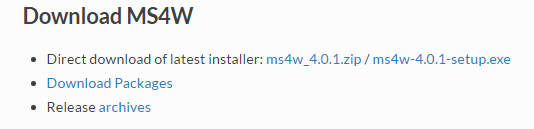
\includegraphics[width=4cm]{figures/tugas4/1174086/download.png}
		\centering
		\caption{Download MS4W}
	\end{figure}
	\hfill\break
	
	\item Setelah download buka aplikasi untuk melakukan instalasi.
\end{enumerate}

\subsection{Konfigurasi Map Server}
Ketika instalasi selesai, lakukan konfigurasi
\begin{enumerate}
	\item Buka folder ms4w pada c:/ms4w. Lalu masuk ke folder apache
	\hfill\break
	
	
	\item Masuk ke folder conf
	\hfill\break
	\begin{figure}[H]
		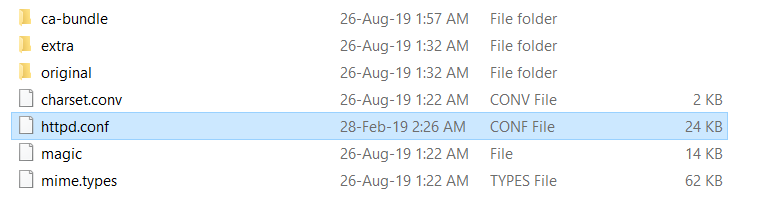
\includegraphics[width=4cm]{figures/tugas4/1174086/conf.png}
		\centering
		\caption{Folder conf}
	\end{figure}
	
	\item Buka file httpd.conf menggunakan sublime lalu cari tulisan Listen. Karena pada komputer saya port 80 digunakan oleh xampp maka saya ubah menjadi 2000.
	\hfill\break
	\begin{figure}[H]
		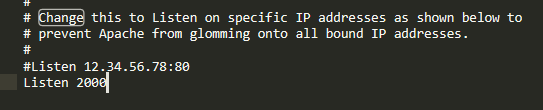
\includegraphics[width=4cm]{figures/tugas4/1174086/2000.png}
		\centering
		\caption{File httpd.conf}
	\end{figure}
	
	\item Kemudian kita restart service milik ms4w dengan cara, membuka task manager
	\hfill\break
	
	\item Lalu pilih Services, cari ApacheMS4WWebServer, kemudian klik kanan lalu restart
	\hfill\break
	
\end{enumerate}


\subsection{Instalasi MapProxy}
\begin{enumerate}
	\item Buka Command Prompt pada Windows
	\item Lalu ketikkan pip install MapProxy
	\hfill\break
	\begin{figure}[H]
		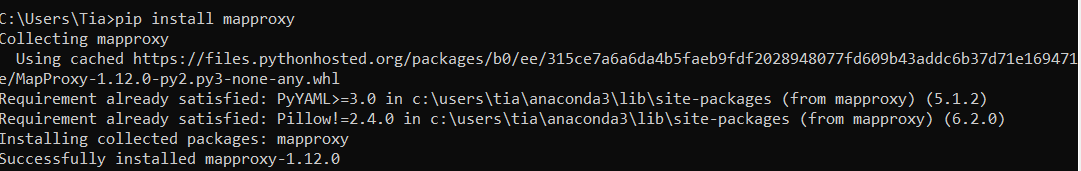
\includegraphics[width=4cm]{figures/tugas4/1174086/mapproxy.png}
		\centering
		\caption{Instalasi MapProxy}
	\end{figure}
\end{enumerate}

\subsection{Membuka map menggunakan MapProxy}
\begin{enumerate}
	\item Download / clone git dari https://github.com/awangga/gede
	\item Path menuju folder gede 
	\item Pada folder gede-master buat folder bernama tmp
	\item Setelah itu buka folder mapproxy lalu edit file agm.yaml
	\item Edit pada bagian sources lalu ada map, masukkan pathnya sesuai dengan dimana menyimpan file gede yang anda telah di clone
	\item Lalu dibawahnya pada bagian binary masukkan lokasi instalasi ms4w, lalu tambahkan /Apache/cgi-bin/mapserv.exe, yang setelah di edit menjadi C:/ms4w/Apache/cgi-bin/mapserv.exe	
	\item Setelah itu buka aplikasi MS4W-Shell, lalu buka lokasi folder gede yang telah di clone
	\item setelah dibuka ketikkan "mapproxy-util serve-develop ./agm.yaml" pada ms4w-Shell untuk membuka aplikasi mapproxy
	\item Buka browser lalu ketikkan 127.0.0.1:8080
	\hfill\break
	\begin{figure}[H]
		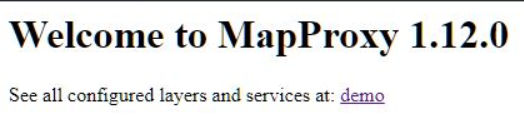
\includegraphics[width=4cm]{figures/tugas4/1174086/buka.png}
		\centering
		\caption{Buka mapproxy pada browser}
	\end{figure}
	
	\item lalu klik demo untuk melihat map
	\item lalu klik png pada agm, maka mapproxy akan menampilkan map
	\hfill\break
	\begin{figure}[H]
		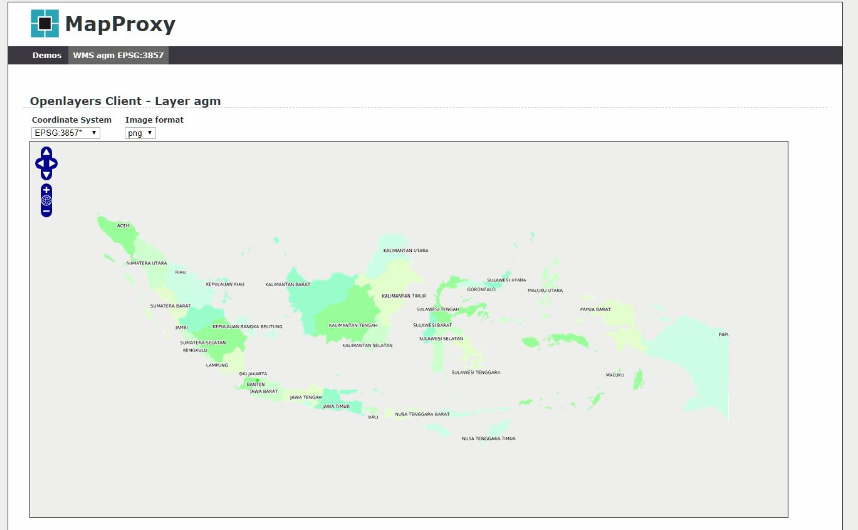
\includegraphics[width=4cm]{figures/tugas4/1174086/peta.png}
		\centering
		\caption{MapProxy menampilkan map}
	\end{figure}
	
\end{enumerate}

\subsection{Link Youtube Instalasi MapServer dan Mapproxy}
https://youtu.be/IXX90Jl6-z4
